\begin{document}

Foi feita uma implementação de um sistema de comunicação utilizando o protocolo LIN, a qual será apresentada em maiores detalhes a seguir. A comunicação acontece entre dois microcontroladores Tiva TM4C123GXL \cite{datasheet:tiva} da Texas Instruments, sendo um mestre e um escravo. Por meio de comunicação serial UART, cada microcontrolador interage com um transceptor LIN no formato de circuito integrado (CI), o MCP2003 \cite{datasheet:mcp2003} fabricado pela Microchip. Por sua vez, os transceptores se comunicam por meio do protocolo LIN, permitindo a troca de mensagens entre mestre e escravo.

Um terceiro microcontrolador foi adicionado -- um Raspberry Pi Pico \cite{datasheet:pico} -- a fim de monitorar a tensão na linha em que acontece a comunicação por LIN. Os dados são obtidos por um conversor analógico-digital (ADC) e salvos em um arquivo no computador.

Os microcontroladores enviam mensagens ao computador no qual estão conectados; portanto, o monitoramento do que é recebido pode ser feito com qualquer software de comunicação serial. O Minicom \cite{minicom} foi utilizado durante os experimentos para esse propósito, bem como para salvar os dados lidos pelo Pi Pico em um arquivo de texto.

O esquemático das conexões feitas pode ser visto na Figura \ref{fig:esquematico}. Nota-se que foi usado um divisor de tensão para as leituras na linha, isso porque o microcontrolador só suporta leituras até 3,3V, mas o LIN opera em 12V. Também, todos os três microcontroladores são alimentados diretamente do computador, porém os transceptores precisam de uma alimentação de, no mínimo, 12V para operar. Assim, uma alimentação externa é feita com duas baterias de 9V usadas e é acondicionada pelos diodos, o capacitor e o diodo Zener. As outras partes do circuito são especificadas pelo \textit{datasheet} do MCP2003.

\begin{figure*}[htb]
    \centering
    \includegraphics[width=.9\textwidth]{../figs/lin-schematic}
    \caption{Esquemático das conexões do experimento.}
    \label{fig:esquematico}
\end{figure*}

Os códigos de cada microcontrolador podem ser encontrados nos Apêndices \ref{master.c} (mestre), \ref{slave.c} (escravo) e \ref{lin-analog.py} (Pi Pico). O código para o responsável por medir a tensão na linha é bastante direto: um \textit{loop} infinito em que ele faz a leitura, quantifica para um intervalo de 0 a 255 e imprime o valor. A impressão é usada para gerar o arquivo com as leituras, e a quantificação é pelo fato de o valor precisar corresponder a um caractere. Já para o mestre e o escravo o código é um pouco mais complexo.

Basicamente, o código implementa a estrutura proposta na Figura \ref{fig:lin_estrutura}, porém com algumas diferenças. O mestre possui um método para enviar o \textit{header} solicitando a mensagem, o qual se repete em até três vezes no caso de a resposta conter algum erro -- identificado pelos métodos de detecção. Esse método é executado periódica e indefinidamente.

No lado do \textit{slave}, um caractere predefinido é enviado juntamente com o CRC do mesmo. Ao final, o \textit{checksum} é enviado normalmente. Com dois métodos de detecção de erro, o sistema ganha uma robustez extra, que é justamente um dos contras desse protocolo. O escravo é ativado por uma interrupção, e caso o destino não seja ele a mensagem é simplesmente ignorada. Já se o ID for o seu, mas os bits de paridade estiverem incorretos, uma resposta errada é enviada para que o mestre possa repetir a solicitação.

As mensagens são enviadas no seguinte formato: primeiro, tanto uma solicitação quanto uma resposta correta devem ser enviadas; depois, o mestre deve enviar o bit de paridade incorreto e, quando então solicitado novamente pelo escravo, enviar o \textit{header correto}; em seguida, o escravo deve enviar três respostas em que o CRC está incorreto; por fim, três respostas em que o \textit{checksum} está incorreto são enviadas. Esse ciclo se repete indefinidamente, permitindo verificar o correto funcionamento de ambos microcontroladores e de todos os métodos de detecção de erro.

A fim de criar um gráfico a partir dos dados obtidos e salvos no arquivo de texto, utilizou-se o código disponível no Apêndice \ref{plot-data.py}. Com ele, uma animação dos dados surge, simulando a execução em tempo real. Sendo assim, uma visualização gráfica do que ocorre na linha é exposta.

O experimento foi construído sobre uma \textit{protoboard}, como mostra a fig \ref{fig:exp}. Um transformador foi posicionado próximo aos componentes para gerar ruído na linha e permitir uma análise do sistema sob condições mais próximas do caso de uso real.

\begin{figure}[H]
    \centering
    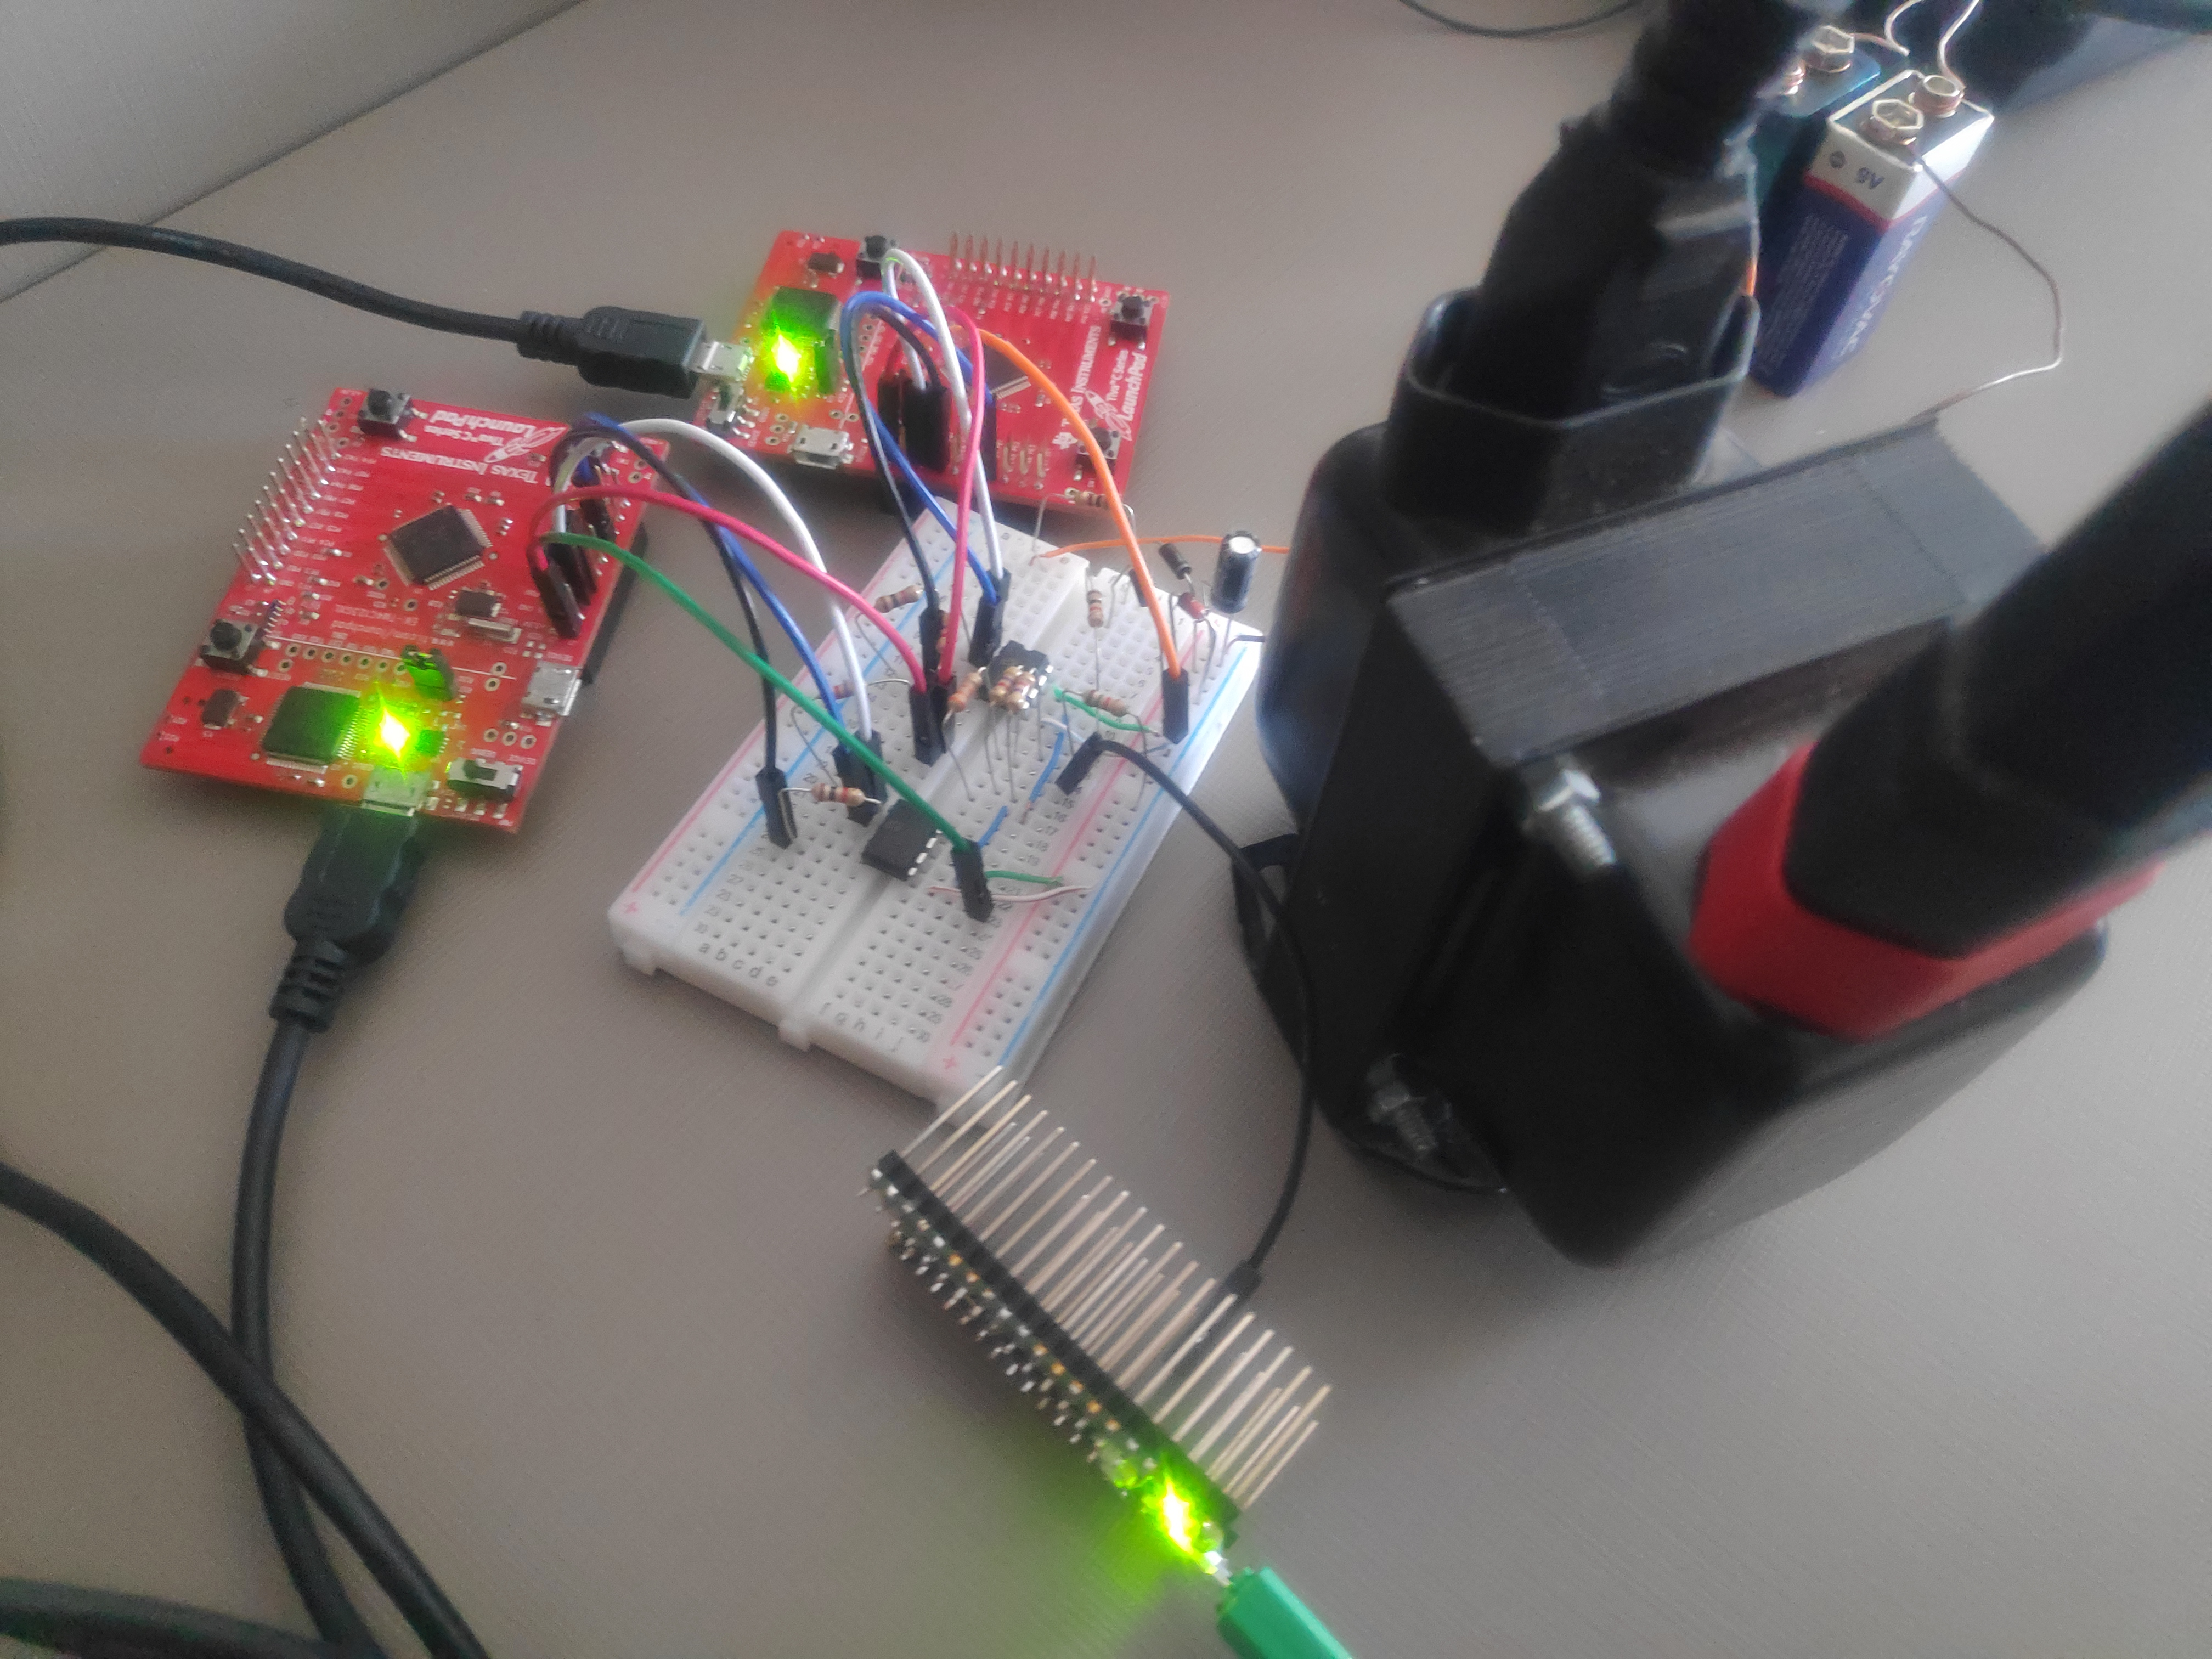
\includegraphics[width=.4\textwidth]{../figs/exp}
    \caption{Imagem do experimento montado.}
    \label{fig:exp}
\end{figure}

Em uma implementação do sistema para um caso de uso real, isto é, em algum subsistema que componha um veículo em produção, algumas partes seriam feitas de maneiras distintas. Por exemplo, a \textit{protoboard} deve ser substituída por uma placa de circuito impresso (PCB), os componentes eletrônicos devidamente ubstituídos e a fonte de alimentação deve ser mais adequada. Todavia, o MCP2003 \cite{datasheet:mcp2003} poderá ser adotado para essa situação, na posição de componente principal da rede.

Com isso, o experimento pode ser construído e testado, gerando dados que permitem avaliar o protocolo de comunicação serial \textit{Local Interconnect Network}. Os resultados obtidos são discutidos na seção seguinte.

\end{document}